\subsection{Рассмотрим игру за студента}
\begin{flushleft}

	Игрок \textbf{С} стремится максимизировать функциональный критерий: 
	
	$$F(x, y) = (\frac{y\sqrt{x}}{2},\frac{\sqrt{1-x}}{y})$$	

	Игрок \textbf{С} использует смешанную стратегию, т.е. его стратегией является
	распределение $q=(q_0,q_1,q_2)$ над множеством чистых стратегий 
	$X=\{0,\frac{1}{2},1\}$:\\

	$$
		F_\textrm{C}=
		\big \langle
			q_0\frac{y\sqrt{0}}{2} + 
			q_1\frac{y}{2} \sqrt{\frac{1}{2}} + 
			q_2\frac{y\sqrt{1}}{2};
			q_0\frac{\sqrt{1}}{y} +
			q_1\frac{1}{y} \sqrt{\frac{1}{2}} +
			q_2\frac{\sqrt{0}}{y}
		\big \rangle = 
	$$
	$$
		=\big \langle
			\frac{y}{2}\cdot\frac{1-q_0+(\sqrt{2}-1)q_2}{\sqrt{2}};
			\frac{1}{y}\cdot\frac{1-q_2+(\sqrt{2}-1)q_0}{\sqrt{2}}
		\big \rangle
	$$	
	
	Затем использует \textbf{ОЛС} (2). Сначала рассмотрим вырожденные случаи \\
	когда $\mu=0$ и  $\mu=1$. 

%-----------------------------------------------------------------------

	\textbf{(1)} Если $\mu=0$:
	$$
		G(y,q,0)=\frac{1}{\sqrt{2}}\cdot \frac{1-q_2+(\sqrt{2}-1)q_0}{y}
	$$	
	
	Далеем осредняем функцию $G(y,q,\mu)$ по стратегиям 
	противника $y \in Y=\{1,2\}$ c вероятностями $(1-p,p)$:
	\begin{gather*}
		\overline G(p,q,0)=
		\frac{1-p}{\sqrt{2}} \cdot \frac{1-q_2+(\sqrt{2}-1)q_0}{1}+
		\frac{p}{\sqrt{2}} \cdot \frac{1-q_2+(\sqrt{2}-1)q_0}{2}=\\
		=\frac{(2-p)(1-q_2+(\sqrt{2}-1)q_0)}{2\sqrt{2}}
	\end{gather*}
	
	Найдём частные производную по переменным $q_0$ и $q_2$, при этом
	введём следующие обозначения для сокращения записи:
	
	\begin{equation}\label{eq:G_dericative}
		\frac{\partial \overline G(p,q,\mu)}{\partial q}
		=\langle \frac{\partial \overline G(p,q,\mu)}{\partial q_0};
		\frac{\partial \overline G(p,q,\mu)}{\partial q_2} \rangle=
		\langle g_1(p,q,\mu), g_2(p,q,\mu) \rangle
	\end{equation}

	$$
		\frac{\partial \overline G(p,q,0)}{\partial q}
		=\frac{2-p}{2\sqrt{2}} \langle \sqrt{2}-1;-1\rangle
	$$
	Поскольку $p \leqslant 1$, то $\dfrac{2-p}{2\sqrt{2}} > 0 $.
	Мы рассматриваем задачу максимизации \\ на множестве $(3)$.
	Следовательно:
	$$q^* = \arg \max \limits_{q \in Q} \overline G(p,q,0)=(1,0).$$

%--------------------------------------------------------------------
	
	\textbf{(2)} Если $\mu=1:$
	$$
		G(y,q,1)=\frac{1}{\sqrt{2}}\cdot \frac{1-q_2+(\sqrt{2}-1)q_0}{y}
	$$	
	
	Далеем осредняем функцию $G(y,q,\mu)$ по стратегиям 
	противника $y \in Y=\{1,2\}$ c вероятностями $(1-p,p)$:
	
	\begin{gather*}
		\overline G(p,q,1)=
		\frac{1-p}{\sqrt{2}} \cdot \frac{1-q_0+(\sqrt{2}-1)q_2}{2}+
		\frac{p}{\sqrt{2}} \cdot \frac{1-q_0+(\sqrt{2}-1)q_2}{1}=\\
		=\frac{(p+1)(1-q_0+(\sqrt{2}-1)q_2)}{2\sqrt{2}}
	\end{gather*}
	
	Найдём частные производную по переменным $q_0$ и $q_2$:	
	
	$$
		\frac{\partial \overline G(p,q,1)}{\partial q}
		=\frac{p+1}{2\sqrt{2}} \langle -1; \sqrt{2}-1\rangle
	$$
	
	Поскольку $p \geqslant 0$, то $\dfrac{p+1}{2\sqrt{2}} > 0 $.
	Мы рассматриваем задачу максимизации \\ на множестве $(3)$.
	Следовательно:
	$$q^* = \arg \max \limits_{q\in Q} \overline G(p,q,1)=(0,1).$$

%--------------------------------------------------------------------
		
	\textbf{(3)} Теперь $\mu \neq 0,1$:
	$$
		G(y,q,\mu)=\frac{1}{\sqrt{2}}\min \limits_{0<\mu<1}
		\big \langle
			\frac{y}{2} \cdot \frac{1-q_0+(\sqrt{2}-1)q_2}{\mu};
			\frac{1}{y} \cdot \frac{1-q_2+(\sqrt{2}-1)q_0}{1-\mu}
		\big \rangle	
	$$

	Далеем осредняем функцию $G(y,q,\mu)$ по стратегиям 
	противника $y \in Y=\{1,2\}$ c вероятностями $(1-p,p)$:

	\begin{multline}\label{eq:G_aver}
		\overline G(p,q,\mu)=\frac{1-p}{\sqrt{2}}\min \limits_{0<\mu<1}
		\big \langle
			\frac{1-q_0+(\sqrt{2}-1)q_2}{2\mu};
			\frac{1-q_2+(\sqrt{2}-1)q_0}{1-\mu}
		\big \rangle + \\
		+\frac{p}{\sqrt{2}}\min \limits_{0<\mu<1}
		\big \langle
			\frac{1-q_0+(\sqrt{2}-1)q_2}{\mu};
			\frac{1-q_2+(\sqrt{2}-1)q_0}{2(1-\mu)}
		\big \rangle 
	\end{multline}
	
	Введём вспомогательные обозначения:
	
	\begin{gather*}
		\ell_1(q,\mu)=\frac{1-q_0+(\sqrt{2}-1)q_2}{2\mu} \\
		\ell_2(q,\mu)=\frac{1-q_2+(\sqrt{2}-1)q_0}{1-\mu} \\
		\ell_3(q,\mu)=\frac{1-q_0+(\sqrt{2}-1)q_2}{\mu} \\
		\ell_4(q,\mu)=\frac{1-q_2+(\sqrt{2}-1)q_0}{2(1-\mu)}
	\end{gather*}
	
	
	Для различных значений переменной $\mu$ рассмотрим 
	взаимные расположения множеств $\ell_1>\ell_2$ и $\ell_3>\ell_4$
	на плоскости $(q_0,q_2)$. Другими словами для фиксированного 
	значения $\mu \in [0,1]$ найдём области плоскости, в которых 
	достигается минимум одного из выражений в (5):
	
	\begin{figure}[H]
    	\centering
     	\begin{subfigure}[b]{0.22 \textwidth}
        	\centering
        	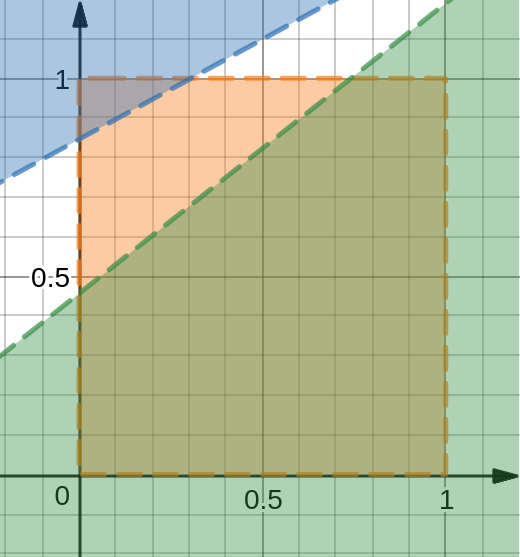
\includegraphics[width=\textwidth]{part_3/graf_6_1}
        	\caption{$\mu=0.8$}
         	\label{fig:y equals x}
     	\end{subfigure}
     	\hfill
     	\begin{subfigure}[b]{0.22 \textwidth}
        	\centering
        	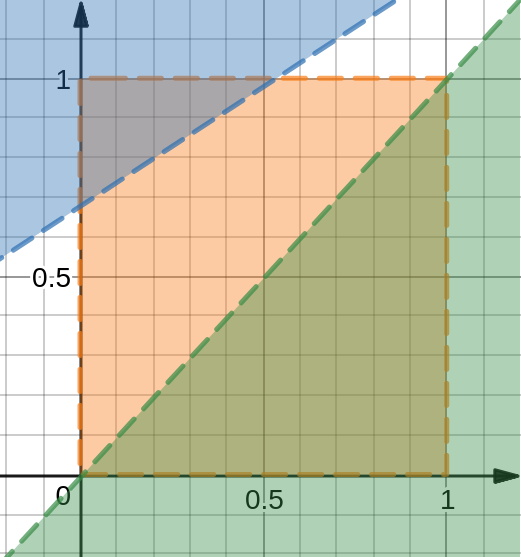
\includegraphics[width=\textwidth]{part_3/graf_6_2}
        	\caption{$\mu=\frac{2}{3}$}
        	\label{fig:three sin x}
     	\end{subfigure}
     	\hfill
     	\begin{subfigure}[b]{0.22 \textwidth}
        	\centering
        	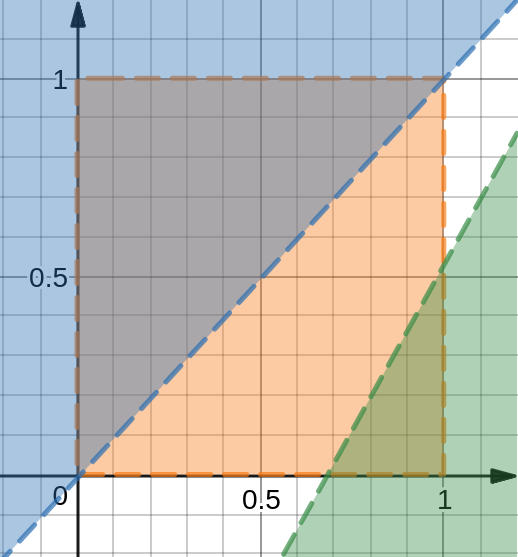
\includegraphics[width=\textwidth]{part_3/graf_6_3}
        	\caption{$\mu=\frac{1}{3}$}
        	\label{fig:five over x}
     	\end{subfigure}
     	\hfill
     	\begin{subfigure}[b]{0.22 \textwidth}
        	\centering
        	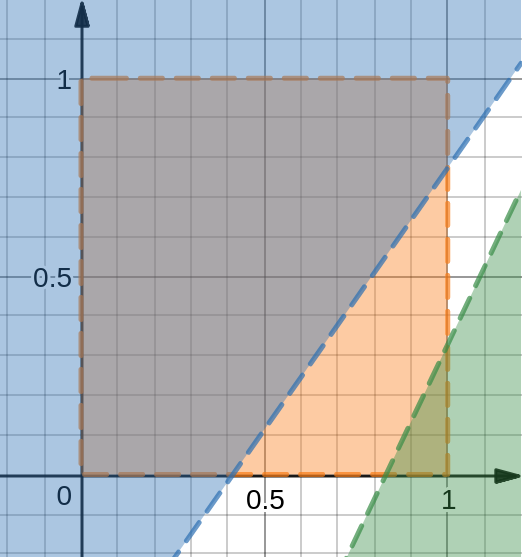
\includegraphics[width=\textwidth]{part_3/graf_6_4}
         	\caption{$\mu=0.1$}
         	\label{fig:five over x}
     	\end{subfigure}
	\end{figure}
	
	Поясним график. Синяя область - это множество $\ell_1 > \ell_2$.\\
	Зелёная область на графике - это множнство $\ell_3 < \ell_4$.\\
	Область между ними - это множество $\{\ell_1<\ell_2 \cap \ell_3 > \ell_4\}$.
	Исходя из графиков $\{\ell_1>\ell_2 \cap \ell_3 < \ell_4\} = \emptyset$ 
	при $(\mu, q) \in (0, 1) \times [0, 1]^2$.
	Поскольку граничные случаи для параметра $\mu$ были рассмотрены в первых
	двух пунктах, то квадрат $[0,1]^2$ на плоскости $(q_0,q_2)$ делится на 3 не 
	пересекающихся множества.
	
	\textbf{Добавить доказательство того, что всего три возможных варианта}

	\textbf{(1)} Рассмотрим полуплоскость, которая определяется системой
	$\begin{cases}
			\ell_1 > \ell_2 \\
			\ell_3 > \ell_4
	\end{cases} \sim \; \l_1 > l_2$
	
	Выражение \eqref{eq:G_aver} на этом множестве принимает следующий вид:
	
	\begin{gather*}
		\overline G(p,q,\mu)=
		\frac{1-p}{\sqrt{2}} \cdot \frac{1-q_2+(\sqrt{2}-1)q_0}{1-\mu} + 
		\frac{p}{\sqrt{2}} \cdot \frac{1-q_2+(\sqrt{2}-1)q_0}{2(1-\mu)} = \\
		=\frac{2-p}{2\sqrt{2}}\cdot\frac{1-q_2+(\sqrt{2}-1)q_0}{1-\mu}		
	\end{gather*}
	
	\textbf{(2)} Рассмотрим полуплоскость, которая определяется системой
	$\begin{cases}
			\ell_1 < \ell_2 \\
			\ell_3 < \ell_4
	\end{cases} \sim \; \l_3 < l_4$
	
	Выражение \eqref{eq:G_aver} на этом множестве принимает следующий вид:
	
	\begin{gather*}
		\overline G(p,q,\mu)=
		\frac{1-p}{\sqrt{2}} \cdot \frac{1-q_0+(\sqrt{2}-1)q_2}{2\mu} + 
		\frac{p}{\sqrt{2}} \cdot \frac{1-q_0+(\sqrt{2}-1)q_2}{\mu} = \\
		=\frac{1+p}{2\sqrt{2}}\cdot\frac{1-q_0+(\sqrt{2}-1)q_2}{\mu}		
	\end{gather*}
	
	\textbf{(3)} Рассмотрим область, которая определяется системой
	$\begin{cases}
			\ell_1 < \ell_2 \\
			\ell_3 > \ell_4
	\end{cases}$

	Выражение \eqref{eq:G_aver} на этом множестве принимает следующий вид:	
	
	\begin{gather*}	
		\overline G(p,q,\mu)=
		\frac{1-p}{\sqrt{2}} \cdot \frac{1-q_0+(\sqrt{2}-1)q_2}{2\mu} +
		\frac{p}{\sqrt{2}} \cdot \frac{1-q_2+(\sqrt{2}-1)q_0}{2(1-\mu)}=\\	
		=\frac{(1-p)(1-\mu)(1-q_0+(\sqrt{2}-1)q_2)+p\mu(1-q_2+(\sqrt{2}-1)q_0)}
		{2\sqrt{2}\mu(1-\mu)}
	\end{gather*}
	
	Итого: 
	
	$$
	\overline G(p,q,\mu) =		
	\begin{cases}
		\dfrac{2-p}{2\sqrt{2}}\cdot\dfrac{1-q_2+(\sqrt{2}-1)q_0}{1-\mu} 
		,\hspace{2mm} \ell_1 \geqslant \ell_2		
		\\
		\dfrac{1+p}{2\sqrt{2}}\cdot\dfrac{1-q_0+(\sqrt{2}-1)q_2}{\mu}
		,\hspace{2mm} \ell_3 \leqslant \ell_4\\
		\dfrac{(1-p)(1-\mu)(1-q_0+(\sqrt{2}-1)q_2)+p\mu(1-q_2+(\sqrt{2}-1)q_0)}
		{2\sqrt{2}\mu(1-\mu)}
		,\hspace{2mm}
		\begin{cases}
			\ell_1 \leqslant \ell_2\\
			\ell_3 \geqslant \ell_4\\
		\end{cases}
	\end{cases}
	$$	
	
	Тогда производная от функции имеет:
	
	$$
	\frac{\partial \overline{G}(p,q,\mu)}{\partial q}=
	\begin{cases}
		\dfrac{2-p}{2\sqrt{2}(1-\mu)} \langle \sqrt{2}-1; -1 \rangle 
 		,\hspace{2mm}
 		\ell_1 \geqslant \ell_2\\
		
		\dfrac{1+p}{2\sqrt{2}\mu} \langle -1; \sqrt{2}-1 \rangle
		,\hspace{2mm}
		\ell_3 \leqslant \ell_4\\
		
		\dfrac{1}{2\sqrt{2}\mu(1-\mu)}
		\big \langle 
			(\sqrt{2} - 1)p\mu -(1-p)(1-\mu);
			(\sqrt{2} - 1)(1-p)(1-\mu) - p\mu			
		\big \rangle
		,\hspace{2mm}
		\begin{cases}
			\ell_1 \leqslant \ell_2\\
			\ell_3 \geqslant \ell_4\\
		\end{cases}
	\end{cases}
	$$
	
%------------------------------------------------------------

	\textbf{(1)} Рассмотрим $\ell_1 \geqslant \ell_2$. 
	Производная в области имеет вид:
	
	$$\frac{\partial \overline{G}(p,q,\mu)}{\partial q}=
	\frac{2-p}{2\sqrt{2}(1-\mu)} \langle \sqrt{2}-1; -1 \rangle$$
 	
	Введём вспомогалетльную функцию	
 	$\ell_B(q, \mu):=(\ell_1-\ell_2) \cdot \mu(1-\mu)$,
 	множество, на котором она принимает неотрицательные значения 
 	составляют интересующую нас область. Множитель $\mu(1-\mu)$ является строго
 	положительным на $\mu \in (0,1)$, поэтому не влияет на знак. Функция
 	является линейной по переменным $q_0$ и $q_2$:
 	
	$$\ell_B(q, \mu) = 
	(1+\mu(2\sqrt{2}-3))q_0+
	(1-\sqrt{2}+\mu(\sqrt{2}-3))q_2
	+3\mu-1$$ 	
	
	Параметр $\mu$ изменяется в диапазоне $(0,1)$, причём	
	
	\begin{gather*}	
	\ell_B(q,\mu) \xrightarrow[\mu\rightarrow 1]{} 
	1-q_0+(\sqrt{2}-1)q_2\\	
	\ell_B(q,\mu) \xrightarrow[\mu\rightarrow 0]{} 	
	1-q_2+(\sqrt{2}-1)q_0\\
	\end{gather*}
	
	Предельные положения $\ell_B(q, \mu)=0$ изображены на графике \eqref{fig:l_B_limits}.
	
	\begin{figure}[H]
		\centering
  		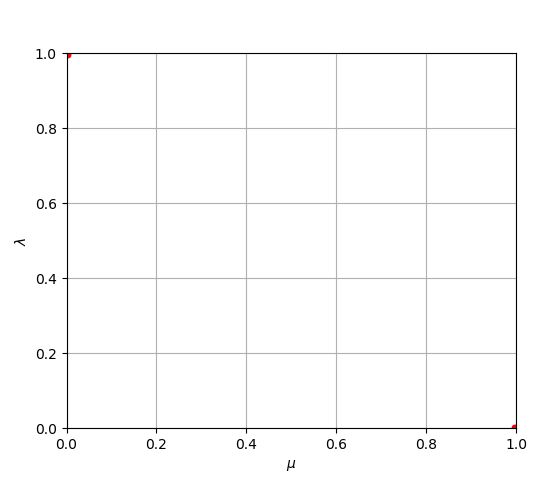
\includegraphics[scale=0.3]{part_3/graf_3_2}
  		\caption{}
  		\label{fig:l_B_limits}
	\end{figure}	
	
	Найдём значение $\mu$ при котором прямая $\ell_B(q, \mu)$ проходит через точку
	$q=(0,0)$:
	
	$$\ell_B(0,0,\hat \mu) = 0
	\Rightarrow \hat \mu = \frac{1}{3}$$	
	
	Очевидно, что на полиэдре $P_B(\mu):$
		
	$$P_B(\mu)=\{q \in Q \; | 
	\;  \ell_B(q, \mu) \geqslant 0 \}, \; \mu \in (0,1)$$
	
	функция $\overline{G}(p,q,\mu)$ достигает максимума в точке $B(\mu):$
	
	$$
	q^* = \arg \max \limits_{q\in P_B(\mu)} \overline G(y,q,\mu) = B(\mu)=
	\begin{cases}
		(0, q_2) : \ell_B(0,q_2,\mu)=0, & \frac{1}{3} \leqslant \mu < 1 \\
		(q_0, 0) : \ell_B(q_0,0,\mu)=0, & 0 < \mu \leqslant \frac{1}{3} \\
	\end{cases}	
	$$
	
	\begin{figure}[H]
    	\centering
     	\begin{subfigure}[b]{0.4 \textwidth}
        	\centering
        	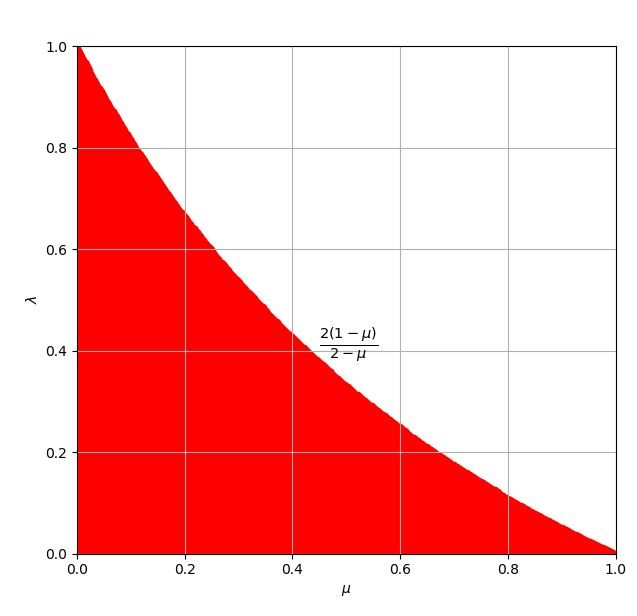
\includegraphics[width=\textwidth]{part_3/graf_3_3}
        	\caption{$\mu=0.1 < \frac{1}{3}$}
         	\label{fig:y equals x}
     	\end{subfigure}
     	\hspace{10mm}
     	\begin{subfigure}[b]{0.4 \textwidth}
        	\centering
        	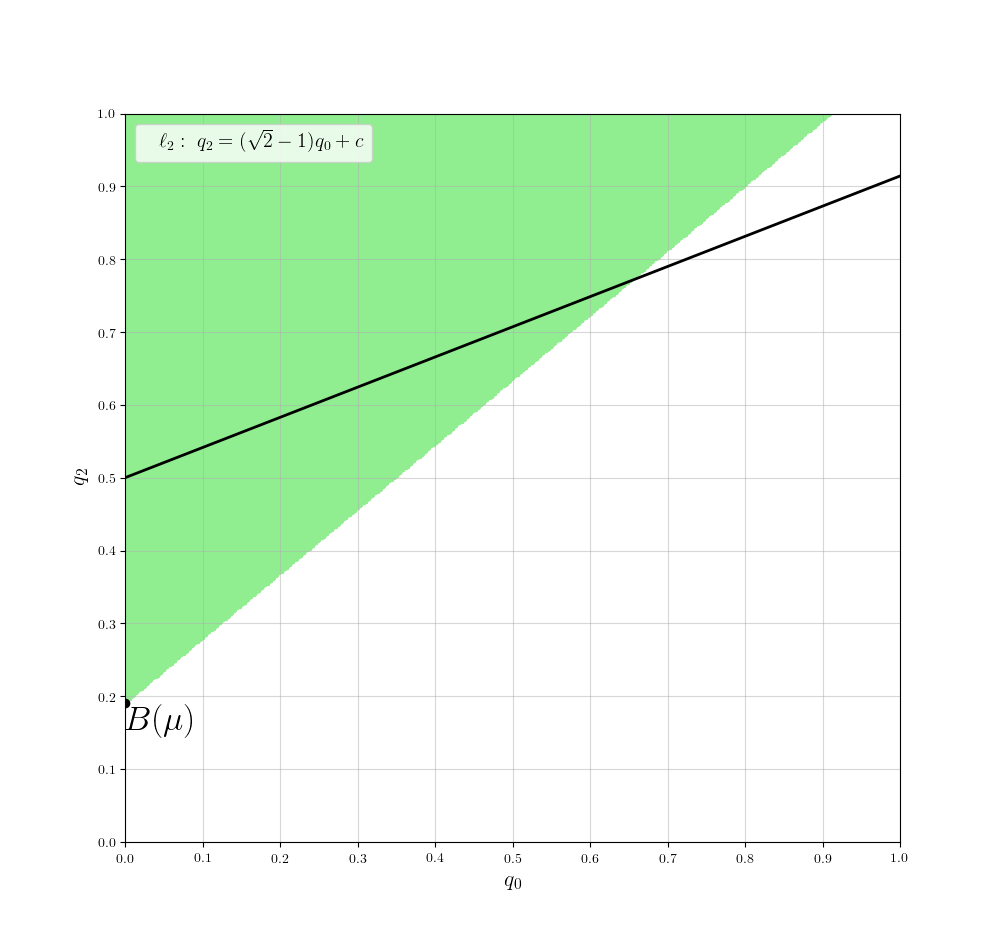
\includegraphics[width=\textwidth]{part_3/graf_3_4}
        	\caption{$\mu=0.4 > \frac{1}{3}$}
        	\label{fig:three sin x}
     	\end{subfigure}
	\end{figure}	

	На графике зелёным цветом изображена область $P_B(\mu)$, чёрным цветом
	обозначены линии уровня и стрелкой соответсвенно градиент функции.
	Рассмотрим эти два случая и найдём явное выражение для точки $B(\mu)$:
	
	\textbf{(a)} Если $\frac{1}{3} \leqslant \mu \leqslant 1$ то координата $q_2$ точки 
	максимума определяется из условия: 
	
	\begin{gather*}
		\ell_B(0,q_2,\mu)=0
		\\
		(1-\sqrt{2}+\mu(\sqrt{2}-3))q_2+3\mu-1=0
		\hspace{3mm} \Rightarrow \hspace{3mm}
		q_2=\frac{3\mu-1}{\sqrt{2}-1+(3-\sqrt{2})\mu}	
		\\
		q^*=(0;\dfrac{3\mu-1}{\sqrt{2}-1+(3-\sqrt{2})\mu}), \hspace{3mm}
		\frac{1}{3} \leqslant \mu \leqslant 1
	\end{gather*}

	\textbf{(b)} Если $0 \leqslant \mu \leqslant \frac{1}{3}$ то координата $q_0$ точки 
	максимума определяется из условия: 	

	\begin{gather*}
		\ell_B(q_0,0,\mu)=0
		\\	
		(1+\mu(2\sqrt{2}-3))q_0
		+3\mu-1=0
		\hspace{3mm} \Rightarrow \hspace{3mm}
		q_0=\frac{1-3\mu}{1+(2\sqrt{2}-3\mu)}	
		\\ 	
		q^*=(\frac{1-3\mu}{1+(2\sqrt{2}-3\mu)}; 0), \hspace{3mm}
		0 \leqslant \mu \leqslant \frac{1}{3}
	\end{gather*}
	
	Следовательно:
	\begin{equation} \label{eq:B}
		B(\mu) = \arg \max \limits_{q\in P_B(\mu)} \overline G(y,q,\mu) = 
		\begin{cases}
			(0;\dfrac{3\mu-1}{\sqrt{2}-1+(3-\sqrt{2})\mu})
			, & \frac{1}{3} \leqslant \mu \leqslant 1
			\\
			(\dfrac{1-3\mu}{1+(2\sqrt{2}-3\mu)};0)
			, & 0 \leqslant \mu \leqslant \frac{1}{3}
		\end{cases}
	\end{equation}

%------------------------------------------------------------

	\textbf{(2)} Рассмотрим $\ell_3 \leqslant \ell_4$.
	Производная в области имеет вид:
	
	$$\frac{\partial \overline{G}(p,q,\mu)}{\partial q}=
	\frac{1+p}{2\sqrt{2}\mu} \langle -1;\sqrt{2}-1 \rangle 
 	$$
 	
	Введём вспомогалетльную функцию	
 	$\ell_A(q, \mu):=(\ell_3-\ell_4) \cdot \mu(1-\mu)$,
 	множество, на котором она принимает неотрицательные значения 
 	составляют интересующую нас область. Множитель $\mu(1-\mu)$ является строго
 	положительным на $\mu \in (0,1)$, поэтому не влияет на знак. Функция
 	является линейной по переменным $q_0$ и $q_2$:
 	
	$$\ell_A(q, \mu)=
	-(2+(\sqrt{2}-3)\mu)q_0
	-(2-2\sqrt{2}+(2\sqrt{2}-3)\mu)q_2
	-3\mu+2$$ 	
 	
	Параметр $\mu$ изменяется в диапазоне $(0,1)$, причём	
	
	\begin{gather*}	
	\ell_A(q,\mu) \xrightarrow[\mu\rightarrow 1]{} 
	1-q_0+(\sqrt{2}-1)q_2\\	
	\ell_A(q,\mu) \xrightarrow[\mu\rightarrow 0]{} 	
	1-q_2+(\sqrt{2}-1)q_0\\
	\end{gather*}
	
	Предельные положения $\ell_B(q, \mu)=0$ изображены на графике \eqref{fig:l_B_limits}.
	Найдём значение $\mu$ при котором прямая 
	$\ell(q, \mu)$ проходит через точку
	$q=(0,0)$:
	
	$$\ell_A(0,0,\hat \mu) = 0 \Rightarrow \hat \mu = \frac{2}{3}$$
	
	Очевидно, что на полиэдре $P_2(\mu):$
	
	$$P_A(\mu)=\{q \in Q \; | 
	\;  \ell_3(q, \mu) \leqslant \ell_4(q, \mu) \}, \; \mu \in (0,1)$$
	
	функция $\overline{G}(p,q,\mu)$ достигает максимума в точке $A(\mu):$
	
	\begin{gather*}
		A(\mu)= \arg \max \limits_{q\in P_A(\mu)} \overline G(p,q,\mu) =
		\begin{cases}
			(0, q_2) : \ell_A(0,q_2,\mu)=0, & \frac{2}{3} \leqslant \mu \leqslant 1 \\
			(q_0, 0) : \ell_A(q_0,0,\mu)=0, & 0 \leqslant \mu \leqslant \frac{2}{3} \\
		\end{cases}		
	\end{gather*}
	
	\begin{figure}[H]
    	\centering
     	\begin{subfigure}[b]{0.45 \textwidth}
        	\centering
        	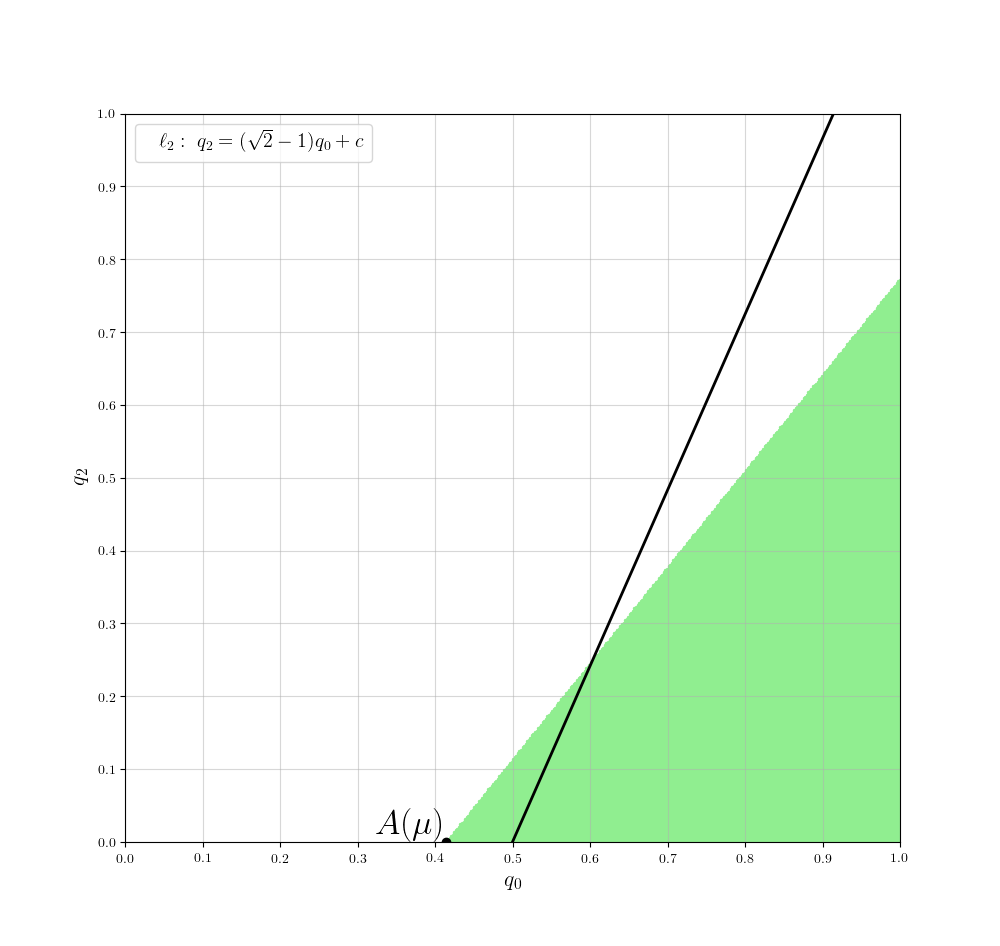
\includegraphics[width=\textwidth]{part_3/graf_3_5}
        	\caption{$\mu=0.1 < \frac{2}{3}$}
         	\label{fig:y equals x}
     	\end{subfigure}
     	\hspace{10mm}
     	\begin{subfigure}[b]{0.45 \textwidth}
        	\centering
        	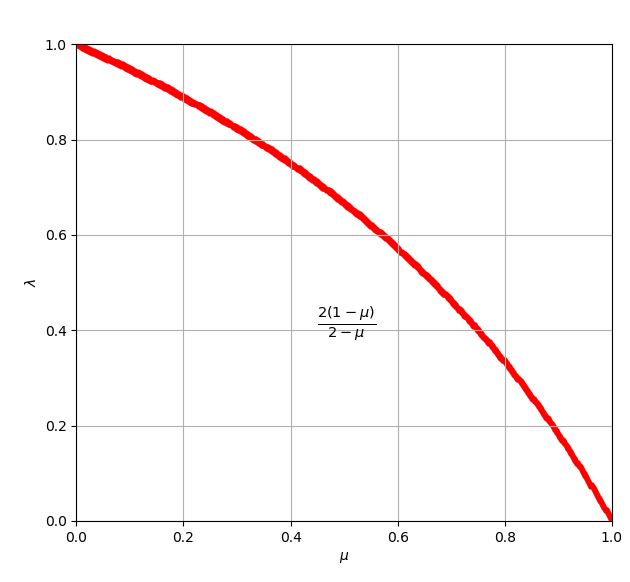
\includegraphics[width=\textwidth]{part_3/graf_3_6}
        	\caption{$\mu=0.8 > \frac{2}{3}$}
        	\label{fig:three sin x}
     	\end{subfigure}
	\end{figure}	
	
	На графике зелёным цветом изображена область $P_A(\mu)$, чёрным цветом
	обозначены линии уровня и стрелкой соответсвенно градиент функции.
	Рассмотрим эти два случая и найдём явное выражение для точки $A(\mu)$:

	\textbf{(a)} Если $\frac{2}{3} \leqslant \mu \leqslant 1$ то координата $q_2$ точки 
	максимума определяется из условия: 	
	
	\begin{gather*}	
		\ell_A(0,q_2,\mu)=0 
		\\
		-(2-2\sqrt{2}+(2\sqrt{2}-3)\mu)q_2
		-3\mu+2=0
		\hspace{3mm} \Rightarrow \hspace{3mm}
		q_2=\frac{3\mu-2}{2(\sqrt{2}-1)+(3-2\sqrt{2})\mu}	
		\\
		q^*= (0;\dfrac{3\mu-2}{2(\sqrt{2}-1)+(3-2\sqrt{2})\mu}), 
		\hspace{5mm} \frac{2}{3} \leqslant \mu \leqslant 1
	\end{gather*}


	\textbf{(b)} Если $0 \leqslant \mu \leqslant \frac{2}{3}$ то координата $q_0$ точки 
	максимума определяется из условия: 	
	
	\begin{gather*}
		\ell_A(q_0,0,\mu)=0	
		\\
		-(2+(\sqrt{2}-3)\mu)q_0
		-3\mu+2=0	
		\hspace{3mm} \Rightarrow \hspace{3mm}
		q_0=\frac{2-3\mu}{2+(\sqrt{2}-3)\mu}	
		\\
		q^*= (\dfrac{2-3\mu}{2+(\sqrt{2}-3)\mu};0), 
		\hspace{5mm} 0 \leqslant \mu \leqslant \frac{2}{3}	
	\end{gather*}
	
	Следовательно:
	\begin{equation} \label{eq:A}
		A(\mu) = \arg \max \limits_{q\in P_A(\mu)} \overline G(p,q,\mu) = 
		\begin{cases}
			(0;\dfrac{3\mu-2}{2(\sqrt{2}-1)+(3-2\sqrt{2})\mu})
			, & \frac{2}{3} \leqslant \mu \leqslant 1 \\
			(\dfrac{2-3\mu}{2+(\sqrt{2}-3)\mu};0), & 0 \leqslant \mu \leqslant \frac{2}{3}	
		\end{cases}
	\end{equation}

%------------------------------------------------------------

	\textbf{(3)} Рассмотрим область в которой
	$\begin{cases}
		\ell_1 \leqslant \ell_2 \\	
		\ell_3 \geqslant \ell_4 \\
	\end{cases}	
	$
	
	Частные производные имеют следующий види в данной области.
	
	$
	\dfrac{\partial \overline{G}(p,q,\mu)}{\partial q}=
	\dfrac{1}{2\sqrt{2}\mu(1-\mu)}
	\big \langle 
		(\sqrt{2} - 1)p\mu -(1-p)(1-\mu);
		(\sqrt{2} - 1)(1-p)(1-\mu) - p\mu			
	\big \rangle
	$

	\begin{gather*}
	g_1=(\sqrt{2} - 1)p\mu -(1-p)(1-\mu) \\
	g_2=(\sqrt{2} - 1)(1-p)(1-\mu) - p\mu
	\end{gather*}

 	Заметим, что функция $\overline{G}(p,q,\mu)$
 	является линейной по переменным $q_0$ и $q_2$ т.е.:

	\begin{gather*}
	\overline{G}(p,q,\mu)=g_0(p,\mu) \: q_0+g_2(p,\mu) \: q_2+c(p,\mu)
	\\
	\textrm{и}
	\\
	\overline{G}(p,q,\mu) = 0 \sim q_2 = k(p, \mu) \cdot q_0 + c(p, \mu)	
	\end{gather*}
	
	Рассматриваем функцию на полиэдре $P_{AB}(\mu):$
	
	$$P_{AB}(\mu)=
	\{
		q \in Q \; | \;  
		\ell_A(q, \mu) \geqslant 0 \cap
	 	\ell_B(q, \mu) \leqslant 0
	\},\; \mu \in (0,1) $$

	Ограничение $\ell_A(q, \mu) = 0$ и $\ell_B(q, \mu) = 0$ представимы в 
	эквивалентном виде:
	
	$$\ell_A(q,\mu)=0 \sim \; q_2=k_A(\mu)q_0+c_A(\mu)$$
	$$\ell_B(q,\mu)=0 \sim \; q_2=k_B(\mu)q_0+c_B(\mu)$$

	
	\begin{figure}[H]
		\centering
  		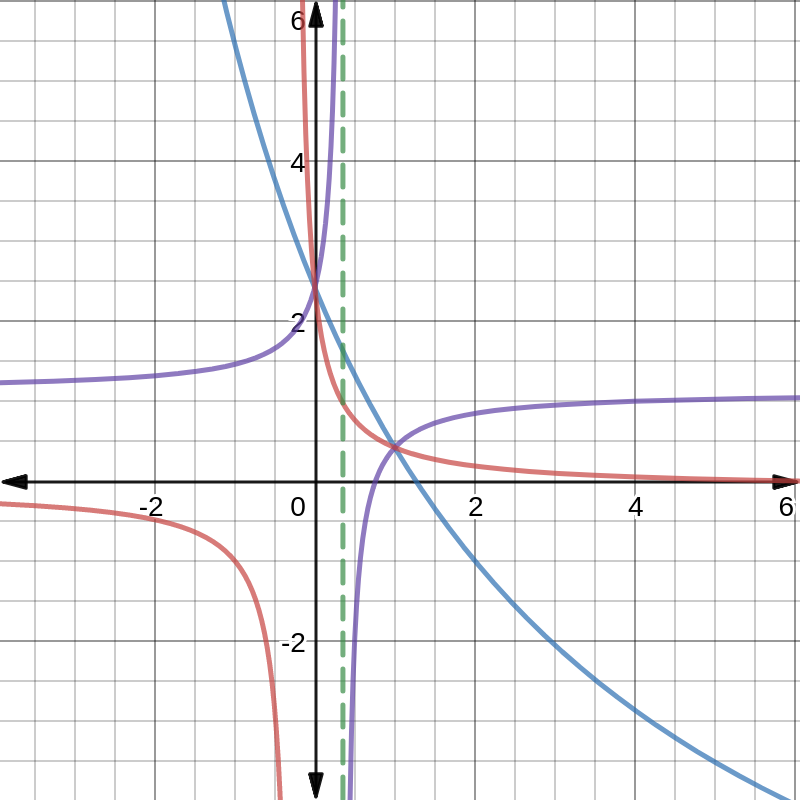
\includegraphics[scale=0.3]{part_3/graf_3_10}
  		\caption{Коэффициенты $k_A(\mu)$, $k_B(\mu)$ и $k(p,\mu)$ при фиксированном $p$}
		\label{fig:k_A,k_B,k}	
	\end{figure}	
	
	Рассмотрим график \ref{fig:k_A,k_B,k}, на котором изображены значения коэффициетов
	при фиксированном значении $p \in [0,1]$. $k_B(\mu)$ изображены красной кривой,
	$k_A(\mu)$ синей и фиолетовой - кривая $k(p, \mu)$. Пунктирная вертикальная линия
	обозначает точку $x$ в которой выражение $g_1=0$. Имеет место неравенство 
	$k_A(\mu) > k_B(\mu)$ при $\mu \in (0,1)$.
	
	$$
	\begin{cases}
	k(\mu) < k_B(\mu) \textrm{ при } g_1(\mu,p) < 0  \\
	k(\mu) > k_A(\mu) \textrm{ при } g_1(\mu,p) > 0 \\
	\end{cases}		
	$$	
	
	
	Следовательно точки максимума функции $\overline{G}(p,q,\mu)$ при фикисированных
	значениях $\mu$ и $p$ могут быть точки: 
	$\{A\}, \{B\}, (0,0)$ и отрезки $[B, A], [0, A], [0,B]$. Где точки
	$A(\mu)$ и $B(\mu)$ определны в \ref{eq:A} и \ref{eq:B}. 
	Рассмотрим три подслучая:
	
	\newpage

	\textbf{(a)} $0 \leqslant \mu \leqslant \frac{1}{3}$. 	
		
	\begin{figure}[H]
    	\centering
     	\begin{subfigure}[b]{0.3 \textwidth}
        	\centering
        	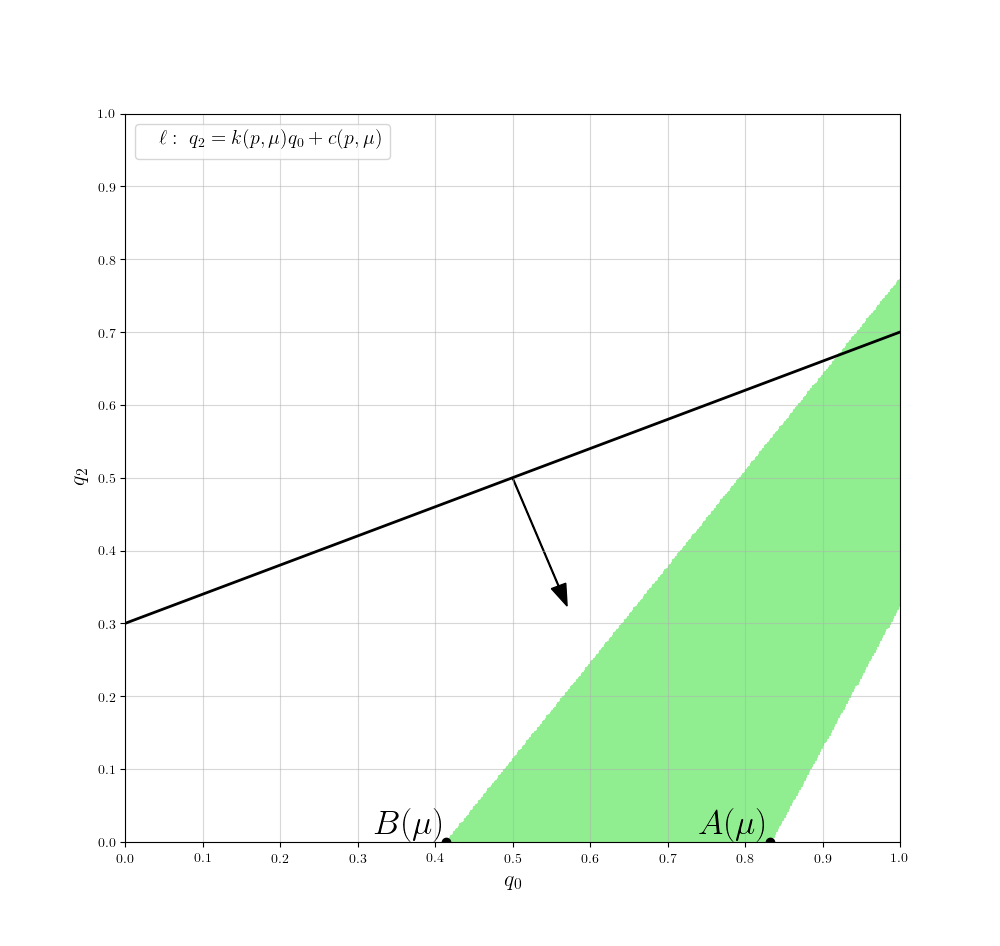
\includegraphics[width=\textwidth]{part_3/graf_3_9_0}
        	\caption{$g_1 > 0 \Rightarrow q^*=A$}
         	\label{fig:y equals x}
     	\end{subfigure}
     	\begin{subfigure}[b]{0.3 \textwidth}
        	\centering
        	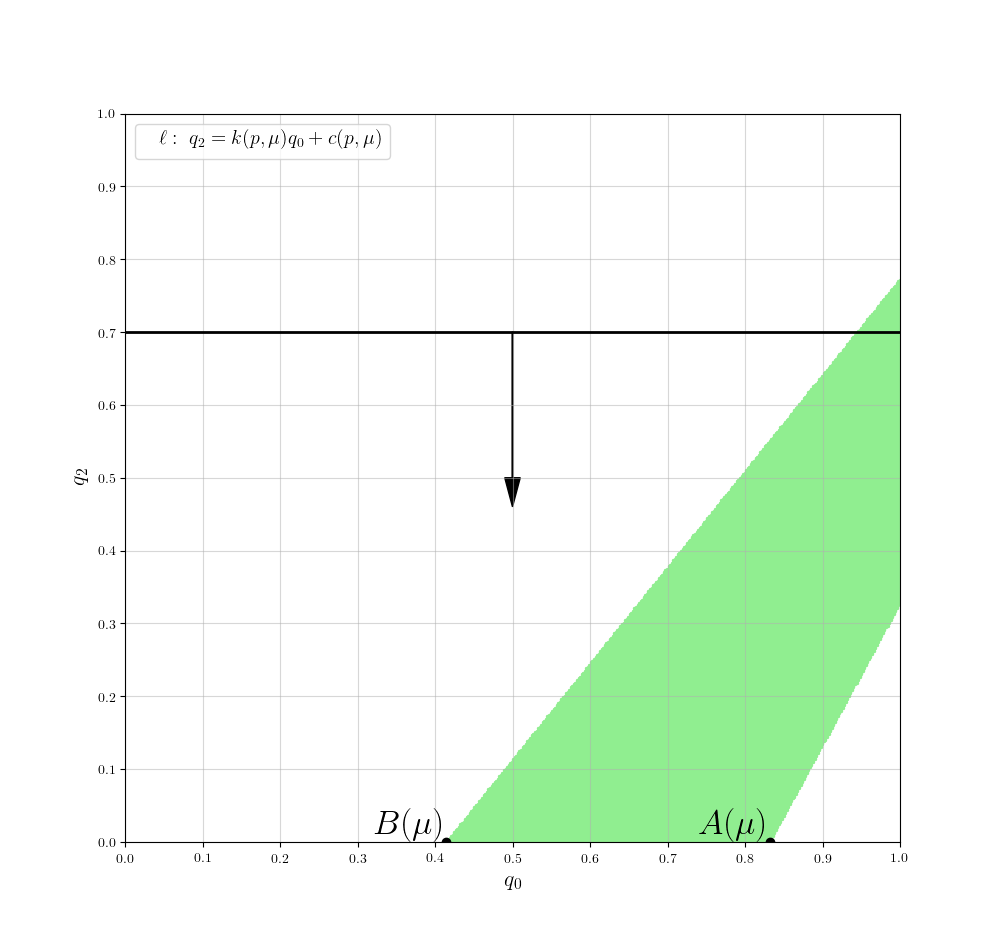
\includegraphics[width=\textwidth]{part_3/graf_3_9_2}
        	\caption{$g_1 = 0 \Rightarrow q^*=[B,A]$}
        	\label{fig:three sin x}
     	\end{subfigure}
     	\begin{subfigure}[b]{0.3 \textwidth}
        	\centering
        	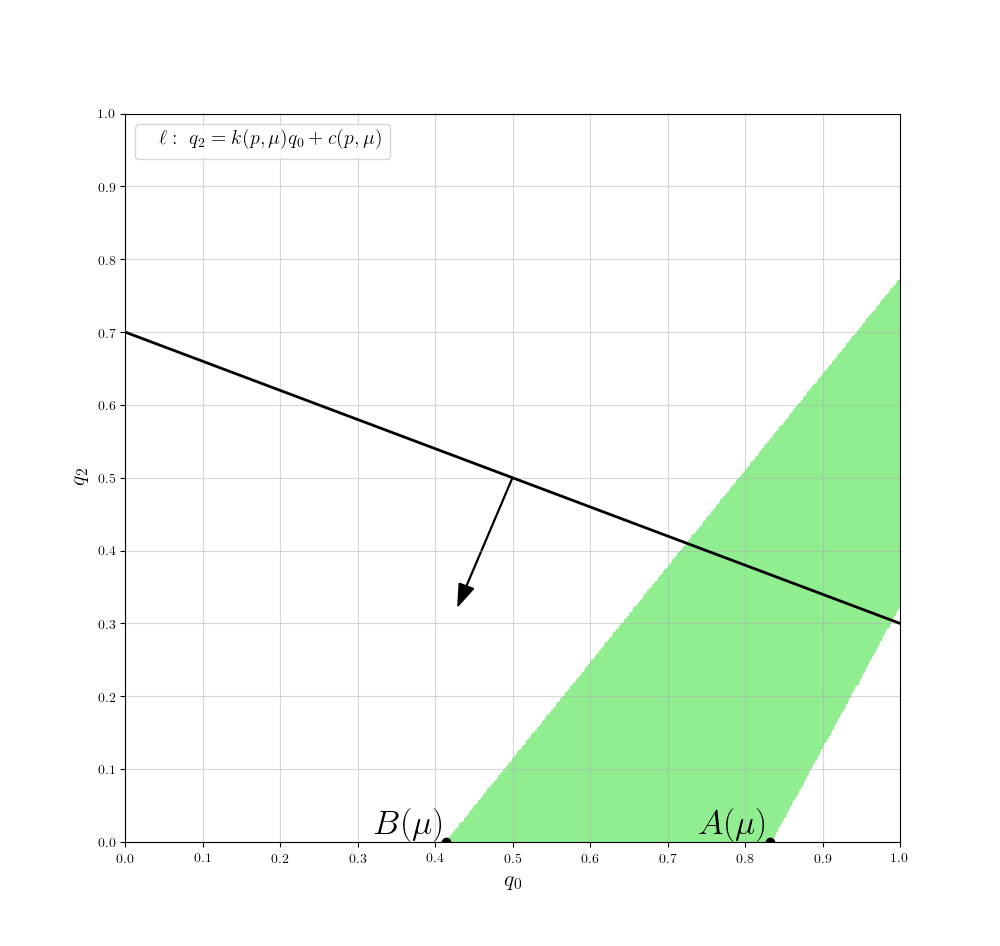
\includegraphics[width=\textwidth]{part_3/graf_3_9_1}
        	\caption{$g_1 < 0 \Rightarrow q^*=B$}
        	\label{fig:three sin x}
     	\end{subfigure}
     	\caption{}
     	\label{fig:3_mu_0}
	\end{figure}

	%Если наклон касательной меньше $k_A$ но больше нуля, то оптимальной точкой
	%является точка $A(\mu)$, если касатальеная паралельна оси $Oq_0$,
	%то множеству оптимальных точек соответсвует отрезок $[B,A]$, если же наклон
	%отрицательный то оптимальной точкой является точка $B(\mu)$.
	%Итого оптимальные точки соответсвуют следующей системе:	
	
	$$
		\begin{cases}
			g_1 > 0 \Rightarrow q^*=A \\
			g_1 = 0 \Rightarrow q^*=[B,A] \\
			g_1 < 0 \Rightarrow q^*=B
		\end{cases}
	$$	
	
	\textbf{(b)} $\frac{2}{3} \leqslant \mu \leqslant 1$
			
	\begin{figure}[H]
    	\centering
     	\begin{subfigure}[b]{0.3 \textwidth}
        	\centering
        	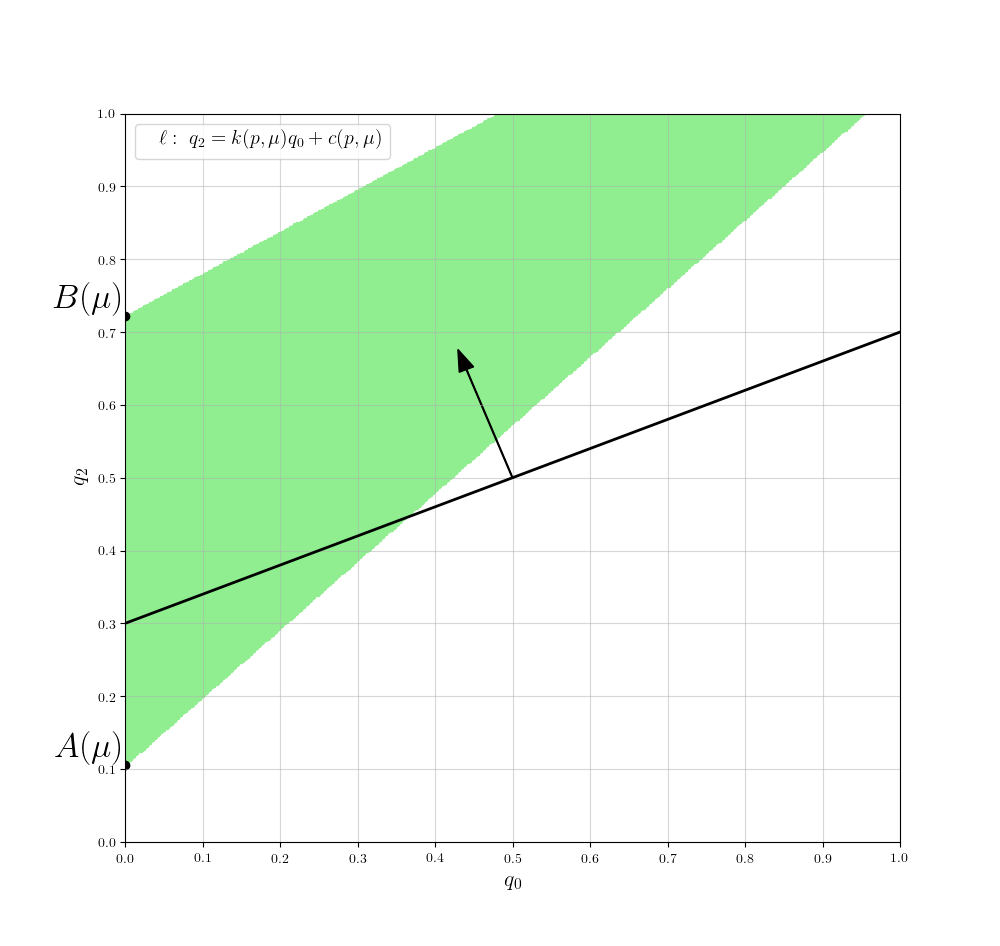
\includegraphics[width=\textwidth]{part_3/graf_3_7_0}
        	\caption{$g_2 > 0 \Rightarrow q^*=B$}
         	\label{fig:y equals x}
     	\end{subfigure}
     	\begin{subfigure}[b]{0.3 \textwidth}
        	\centering
        	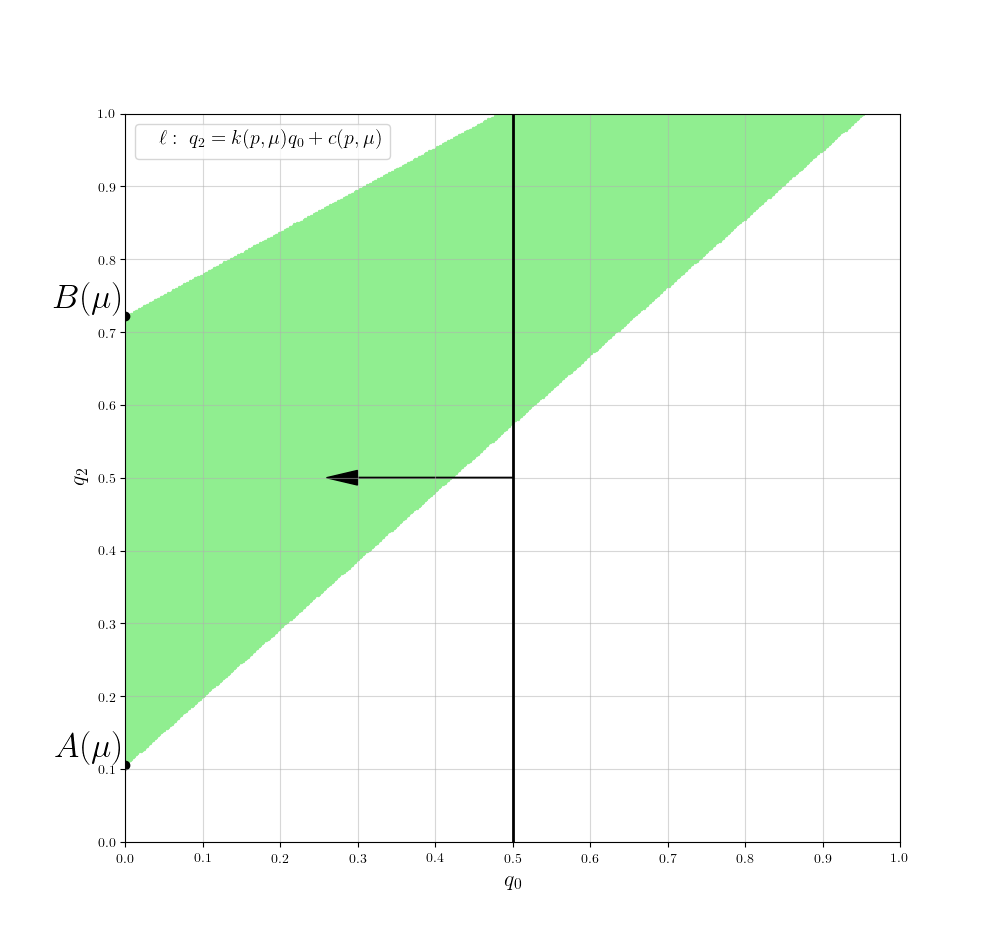
\includegraphics[width=\textwidth]{part_3/graf_3_7_1}
        	\caption{$g_2 = 0 \Rightarrow q^*=[B,A]$}
        	\label{fig:three sin x}
     	\end{subfigure}
     	\begin{subfigure}[b]{0.3 \textwidth}
        	\centering
        	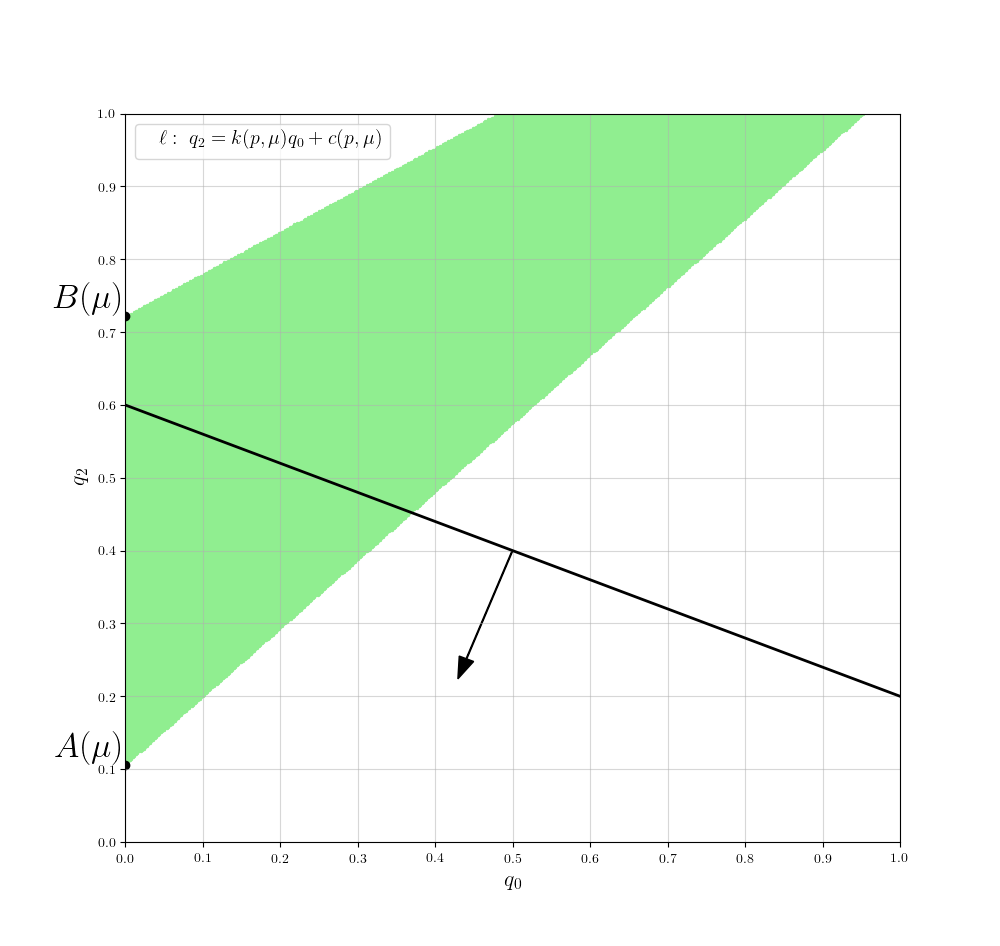
\includegraphics[width=\textwidth]{part_3/graf_3_7_2}
        	\caption{$g_2 < 0 \Rightarrow q^*=A$}
        	\label{fig:three sin x}
     	\end{subfigure}
     	\caption{}
	\end{figure}
	
	\begin{center}
		$\left[
		\begin{gathered}
			g_2 > 0 \Rightarrow q^*=B \\
			g_2 = 0 \Rightarrow q^*=[B,A] \\
			g_2 < 0 \Rightarrow q^*=A
		\end{gathered}
		\right.$	
	\end{center}	
	
	\newpage

	\textbf{(c)} $\frac{1}{3} \leqslant \mu \leqslant \frac{2}{3}$
	
	\begin{figure}[H]
    	\centering
     	\begin{subfigure}[b]{0.3 \textwidth}
        	\centering
        	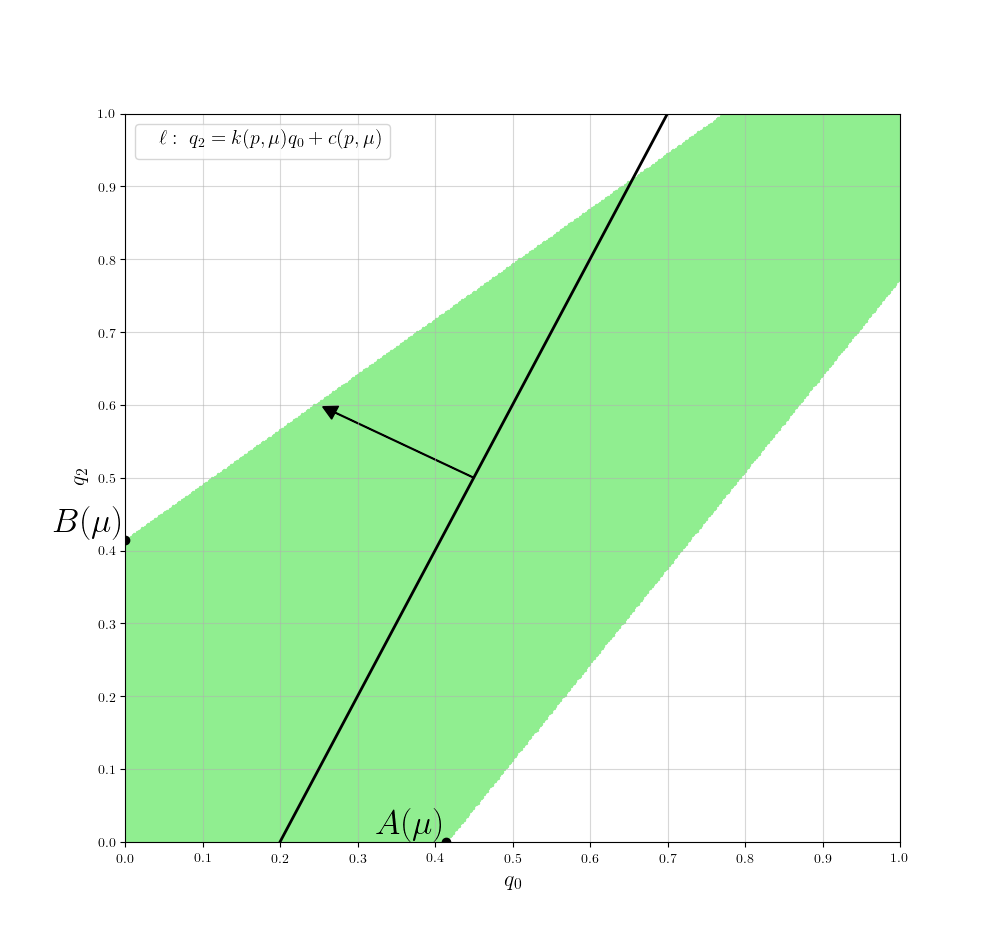
\includegraphics[width=\textwidth]{part_3/graf_3_8_1}
        	\caption{$g_2 > 0 \Rightarrow q^*=B$}
     	\end{subfigure}
     	\begin{subfigure}[b]{0.3 \textwidth}
        	\centering
        	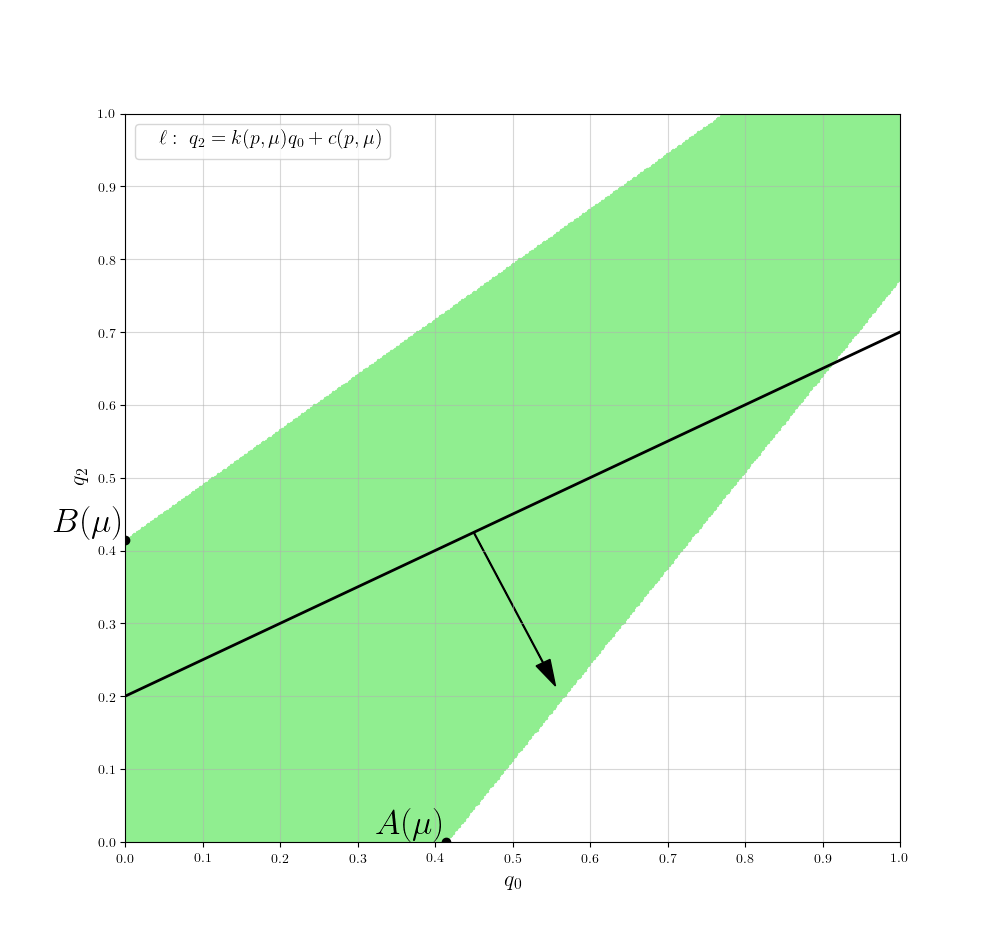
\includegraphics[width=\textwidth]{part_3/graf_3_8_2}
        	\caption{$g_1 > 0 \Rightarrow q^*=A$}
     	\end{subfigure}
     	\begin{subfigure}[b]{0.3 \textwidth}
        	\centering
        	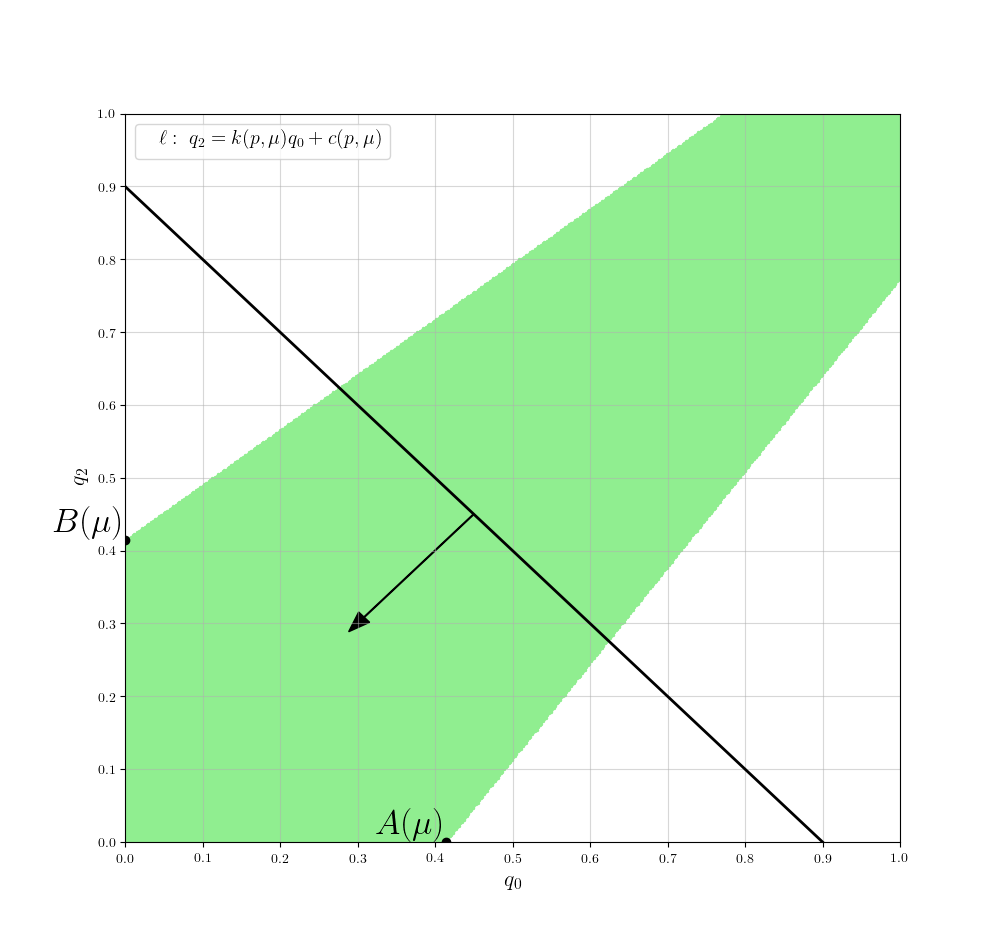
\includegraphics[width=\textwidth]{part_3/graf_3_8_0}
        	\caption{$
        	\begin{cases}			
				g_2 < 0 \\
				g_1 < 0
			\end{cases}	\Rightarrow q^*=(0,0)
			$}
     	\end{subfigure}
    	\centering
     	\begin{subfigure}[b]{0.3 \textwidth}
        	\centering
        	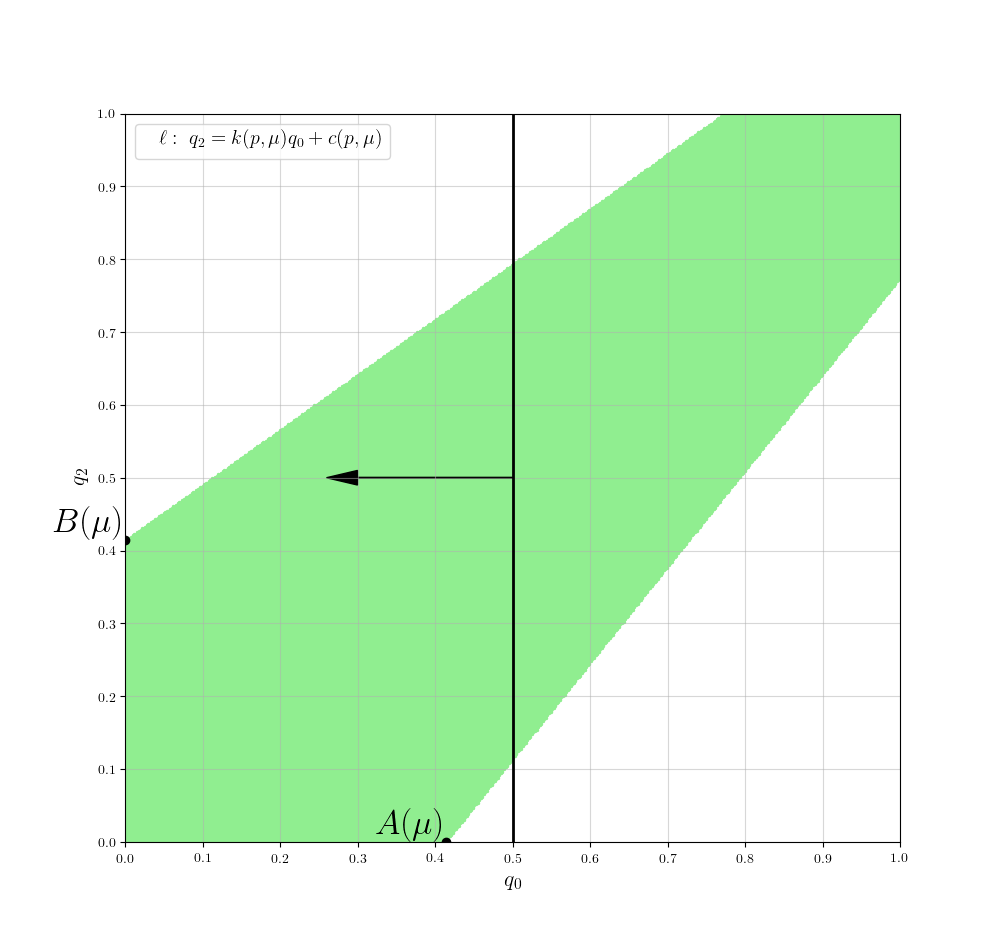
\includegraphics[width=\textwidth]{part_3/graf_3_8_3}
        	\caption{$g_2 = 0 \Rightarrow q^*=[0,B]$}
     	\end{subfigure}
     	\begin{subfigure}[b]{0.3 \textwidth}
        	\centering
        	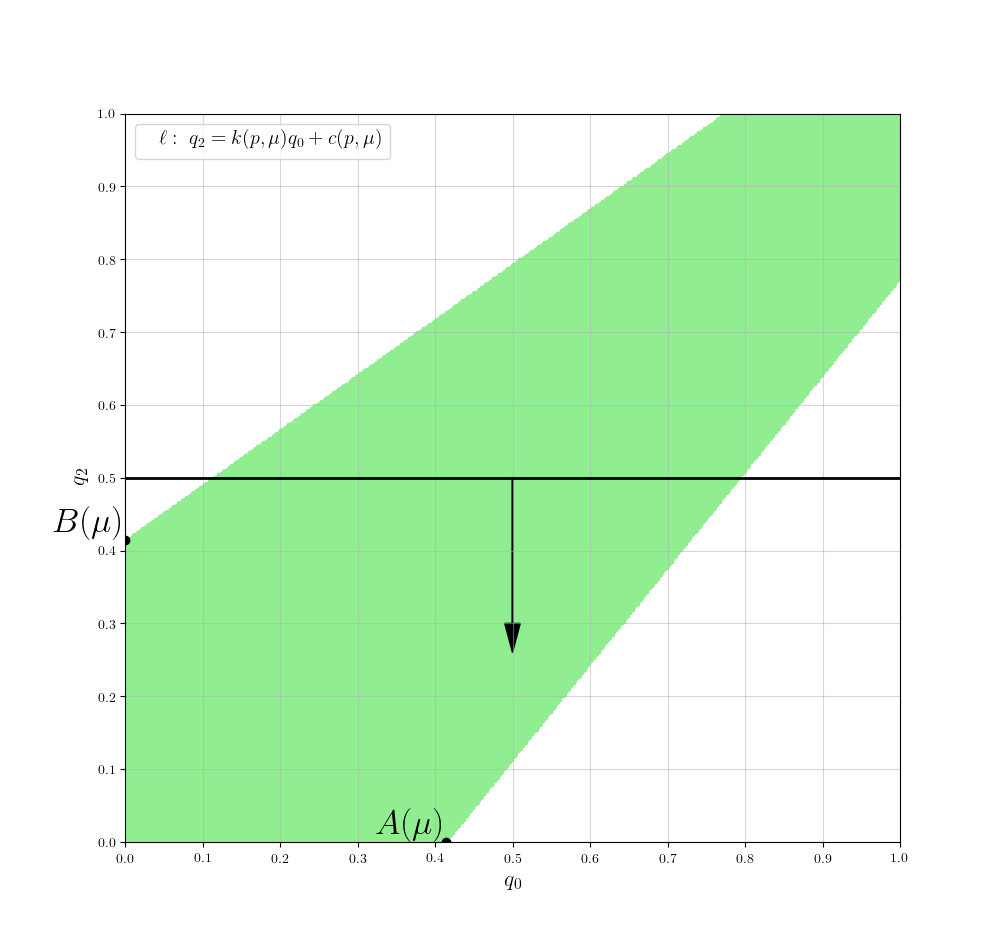
\includegraphics[width=\textwidth]{part_3/graf_3_8_4}
        	\caption{$g_1 = 0 \Rightarrow q^*=[0,A]$}
     	\end{subfigure}
	\end{figure}


	
	\begin{center}
		$\left[
		\begin{gathered}
			g_1 > 0 \Rightarrow q^*=A \\
			g_2 > 0 \Rightarrow q^*=B \\			
			g_1 = 0 \Rightarrow q^*=[0,A] \\
			g_2 = 0 \Rightarrow q^*=[0,B] \\			
			\begin{cases}			
				g_2 < 0 \\
				g_1 < 0
			\end{cases}	\Rightarrow q^*=(0,0)
		\end{gathered}
		\right.$	
	\end{center}

%-------------------------------------------------------------

	Итого получим следующие 

	$C(p,\mu) = \arg \max \limits_{P_{AB}} \overline{G}(p,q,\mu)
	\begin{cases}
	A(\mu), & g_2(p,\mu)<0 \cup \mu \leqslant \frac{1}{3} \cap g_2 < 0 \\
	B(\mu), & g_1(p,\mu)>0 \cup \mu \geqslant \frac{2}{3} \cap g_1 > 0 \\
	(0,0),  & g_1(p,\mu)<0 \cap g_2(p,\mu)<0 \\
	[A(\mu), B(\mu)], 
	& g_1(\mu)=0 \cap \mu < \frac{1}{3} \cup g_1(\mu)=0 \cap \mu > \frac{2}{3} \\
	[0, A(\mu)], & g_2(\mu)=0 \cap \mu \in [\frac{1}{3},\frac{2}{3}] \\
	[0, B(\mu)], & g_1(\mu)=0 \cap \mu \in [\frac{1}{3},\frac{2}{3}] \\
	\end{cases}	
	$	
	
	Но кроме того точки $A(\mu)$ и $B(\mu)$ являются оптимальными 
	$\forall$ $p$ и $\mu$ поскольку	являются таковыми в \textbf{(1)} и \textbf{(2)}.
	Итого в области $P_B$ оптимальной является точка $B(\mu)$,
	в области $P_A$ оптимальной является точка $A(\mu)$,
	и в области $P_{AB}$ оптимальной является точка $C(p, \mu)$.
	Поскольку если $f(x)$ и $g(x)$ непрерывны на множестве $X$, то и 
	$min(f(x), g(x))$ непрерывна на $X$, то максимум достигается в точке
	$C$.
	
	$q^*(p,\mu)= \arg \max \limits_Q \overline{G}(p,q,\mu)
	\begin{cases}
	A(\mu), & g_2(p,\mu)<0 \cup \mu \leqslant \frac{1}{3} \cap g_2 < 0 \\
	B(\mu), & g_1(p,\mu)>0 \cup \mu \geqslant \frac{2}{3} \cap g_1 > 0 \\
	(0,0),  & g_1(p,\mu)<0 \cap g_2(p,\mu)<0 \\
	[A(\mu), B(\mu)], 
	& g_1(\mu)=0 \cap \mu < \frac{1}{3} \cup g_1(\mu)=0 \cap \mu > \frac{2}{3} \\
	[0, A(\mu)], & g_2(\mu)=0 \cap \mu \in [\frac{1}{3},\frac{2}{3}] \\
	[0, B(\mu)], & g_1(\mu)=0 \cap \mu \in [\frac{1}{3},\frac{2}{3}] \\
	(0,1), & \mu = 0 \\
	(1,0), & \mu = 1
	\end{cases}	
	$		
	
	
	%$$g_1=p\mu-(1-p)(1-\mu)  \hspace{10mm}
	%g_1=0 \sim p=\frac{1-\mu}{(\sqrt{2}-2)\mu + 1}$$

	%$$g_2=(1-p)(1-\mu)(\sqrt{2}-1)-p\mu  \hspace{10mm}
	%g_2=0 \sim p=\frac{(1-\mu)(\sqrt{2}-1)}{(\sqrt{2}-2)\mu + (\sqrt{2}-1)}$$
	
	Поскольку в пункте 3.1 мы установили, что 
	
	$$p^*(q,\lambda(q))=\arg \max \limits_{p \in [0,1]}
		\overline{L}(p, q, \lambda(q))=[0,1]
	$$

	Нас интересуют оптимальные пары $(p^0,q^0)$ такие, что 
	$\exists (\lambda, \mu) \in [0,1]^2 $:
	
	$$\begin{cases}
	p^0=p^*(q^0,\lambda) \\
	q^0=q^*(p^0,\mu)
	\end{cases}$$
	
	Введём следующие множества:
	
	$$P_0=[0,1], \; Q_0=\{(q_0,q_2) \in Q \: | \: q_0=0 \textrm{ или } q_2 = 0\}$$
	
	Следующие точки являются оптимальными:
	$$(p, q) \in P_0 \times Q_0$$
		

\end{flushleft}



















